\subsection{Réseau}

    \subsubsection{Création d'une salle}
        Photon se base sur un système de salle. Ces dernières permettent aux joueurs présent à l'intérieur de communiquer entre eux. Il est actuellement possible de créer ainsi que de rejoindre une salle. Ces deux processus se font automatiquement, sans effort du joueur, mais il est prévu de donner un plus grand contrôle sur ce système aux clients. En effet, il suffit d'appuyer sur un bouton pour tenter de rejoindre une salle. Si aucune salle est disponible, alors le client en crée une qui se rend disponible aux autres joueurs. Ce système a été implémenté par Julien et Harrys.
    \subsubsection{Instantiation et synchronisation}
        C'est Harrys qui s'est occupé de cette partie. Une fois que le joueur accède à une salle, celui-ci charge une scène, la même que tout les autres joueurs. Photon permet alors d'instancier son personnage, qui sera visible par tout les autres joueurs présent dans la salle.
        Cependant cela ne suffit pas, car il faut ensuite permettre la synchronisation des mouvements des joueurs. Pour celà, on utilise un composant appelé PhotonView. Ce dernier permet de synchroniser divers variables spécifiques à un objet comme sa position ou ses animations. De plus ce composant est nécessaire pour la communciation par "RPC" qui est essentiel à la réalisation du multijoueur.
        Certains éléments, tels que ceux permettant de contrôler le personnage grâce à l'utilisation du clavier ou bien d'une manette, doivent cependant être pris en compte lors de ce processus. Chaque client doit désactiver les composants problématiques des personnages qu'il ne "possède" pas. On utilise le système d'appartenance d'objet qui, tout comme la synchronisation de mouvement, se fait grâce au composant PhotonView.
        La scène actuel d'instantiation servant de lobby, divers ajouts "cosmétiques" ont été effectués comme l'apparition des pseudos au dessus de chaque joueur ou bien l'implémentation du choix de l'apparence.
        Un système de "timer", synchronisé pour tout les joueurs d'une salle est actuellement en cours de développement.
        Par la suite, les différentes actions pouvant être réalisés par les joueurs devront également être synchronisés. Cepdendant le travail effectué jusqu'à présent facilitera grandement cette tâche.
        
        \begin{figure}[!hbt]
                \centering 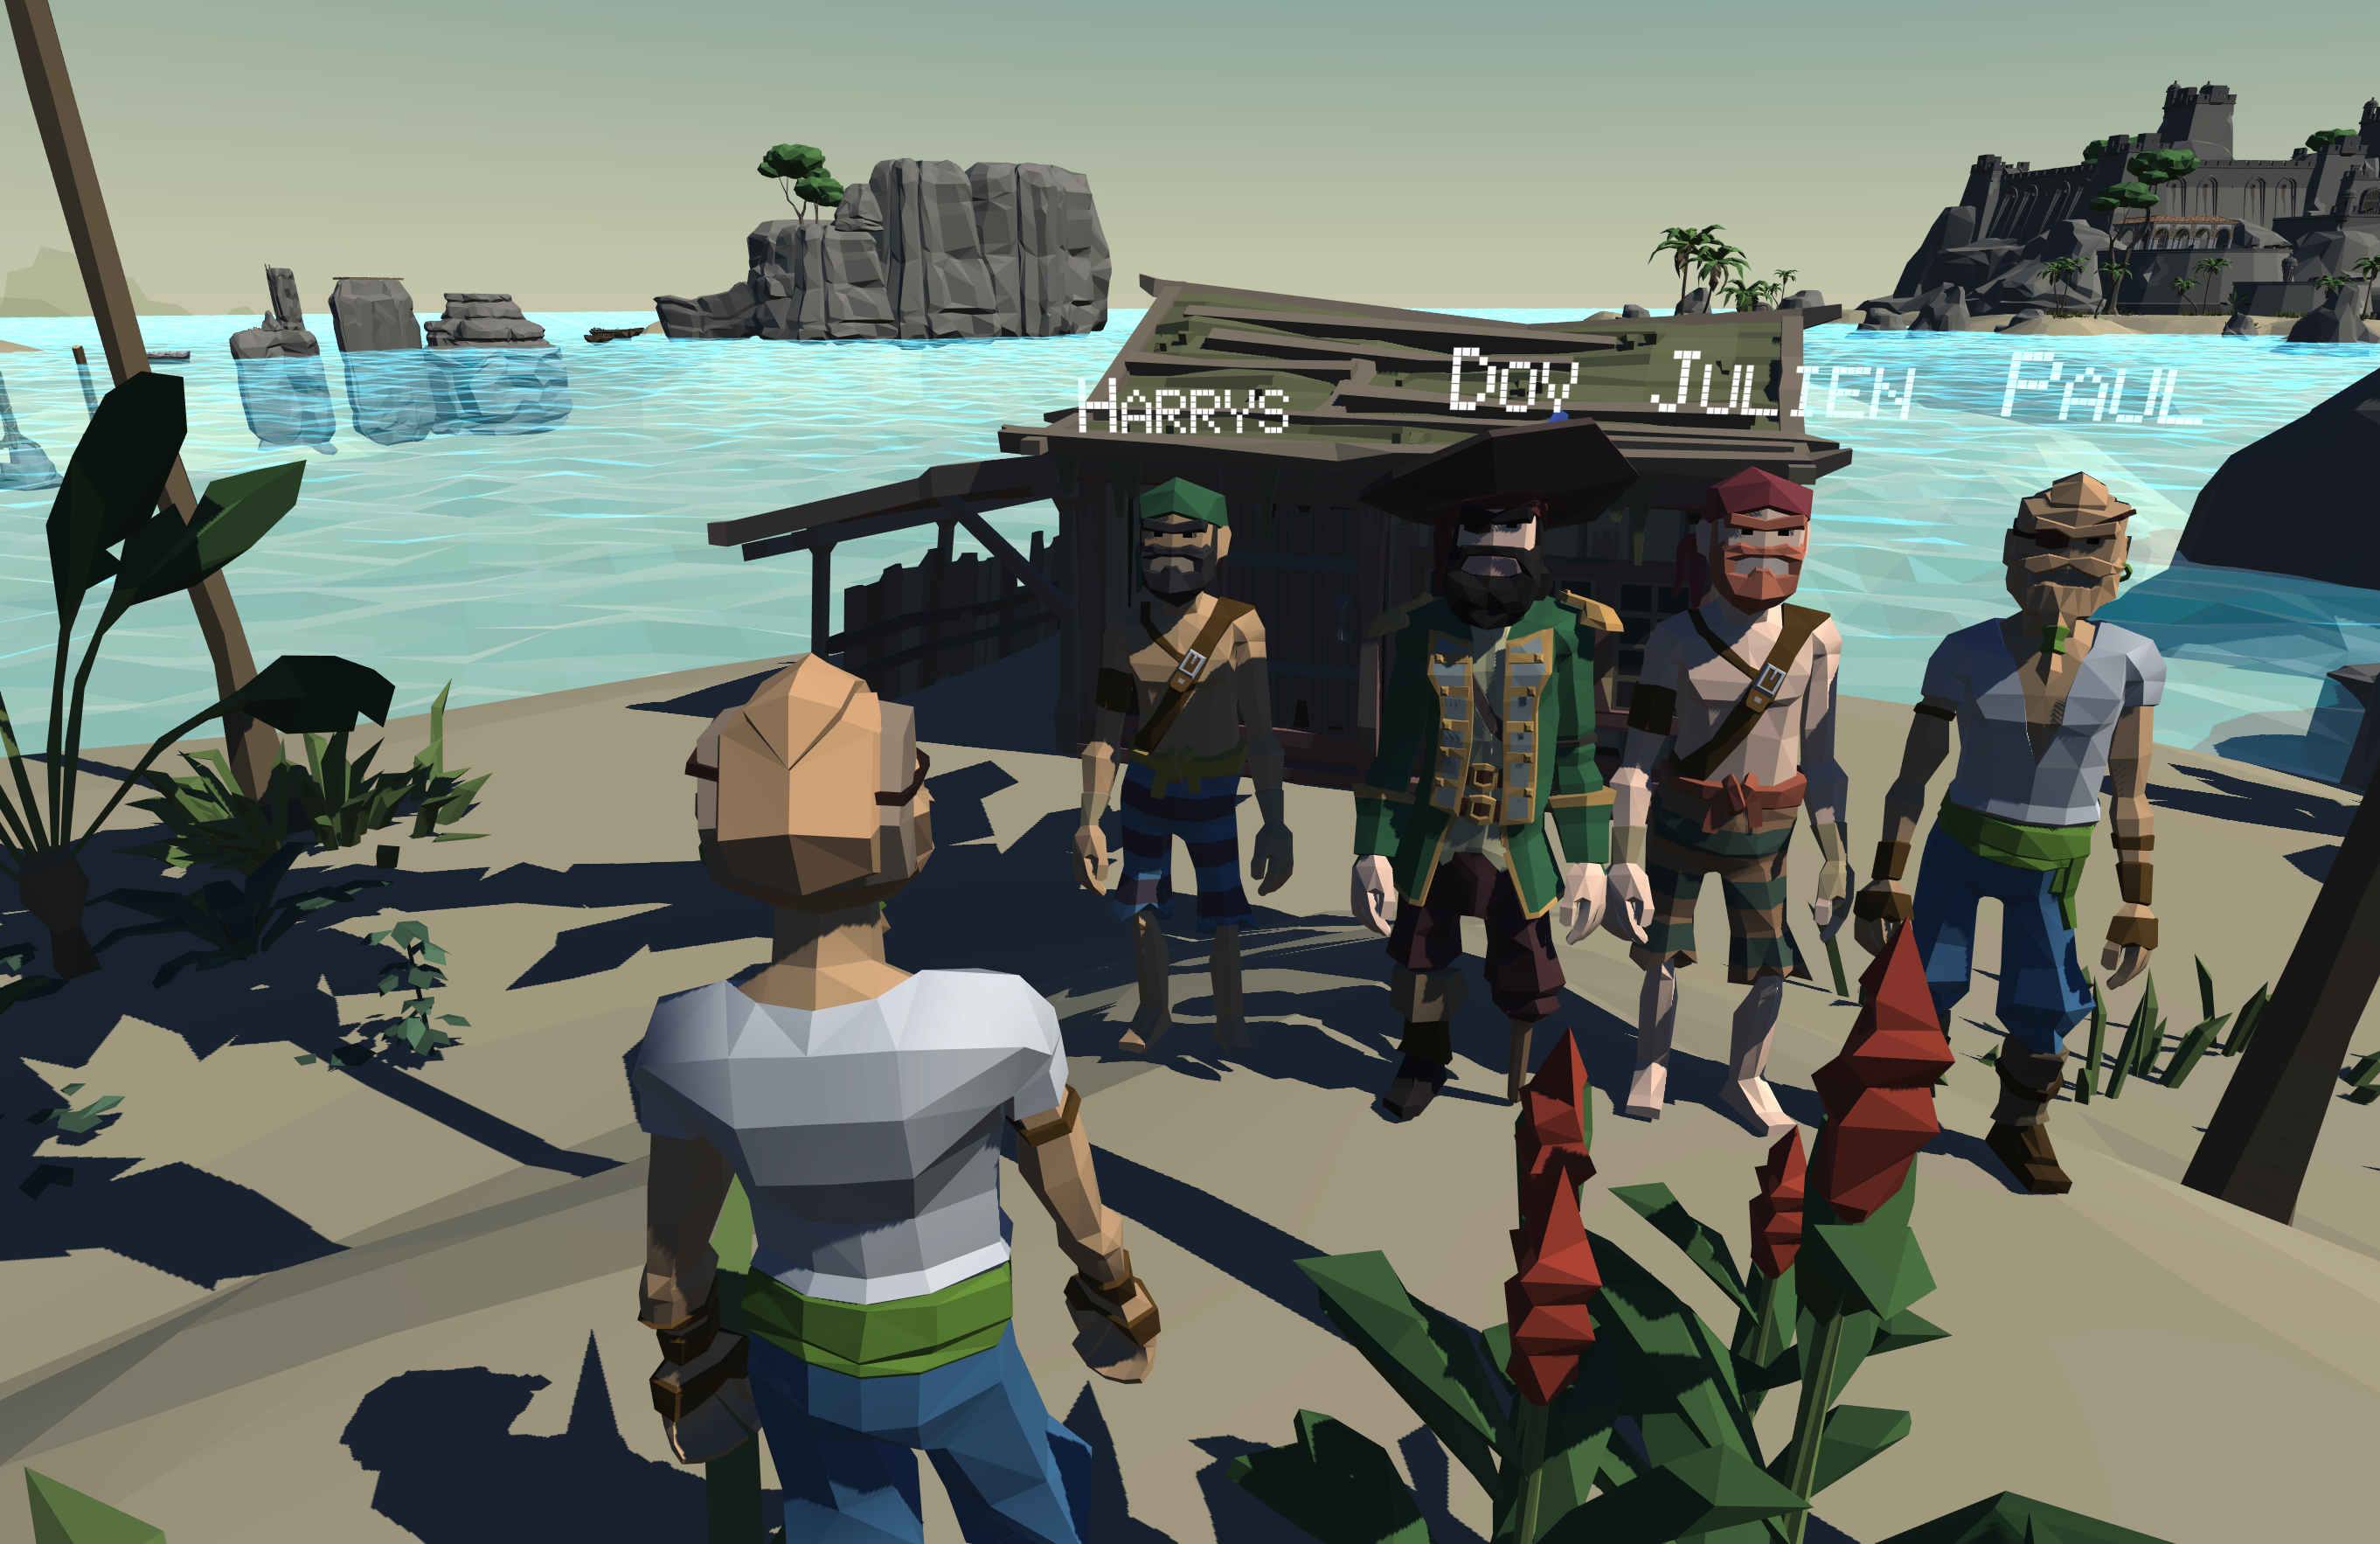
\includegraphics[scale=0.2]{in_game_lobby.png} 
                \caption{Photo de groupe en multijoueur}
            \end{figure}